% resultados

\chapter{Resultados}

Nesta parte serão apresentados os resultados obtidos através da abordagem metodológica abordada anteriormente. Na Seção \ref{section:estat_desc} são abordadas estatísticas descritivas acerca das atas do Copom. Já na Seção \ref{section:indice_sentimentos} é abordado o índice de sentimentos criado e comparação dele com as variáveis macroeconômicas presentes neste trabalho. Na Seção \ref{section:testes_estac} são expostos os resultados dos testes de estacionariedade para as variáveis macroeconômicas e para o índice. Por fim, a Seção \ref{section:VAR} trata da modelagem econométrica, onde por meio da aplicação de VAR, obtém-se as IRF.

\section{Estatísticas descritivas} \label{section:estat_desc}

Com os dados limpos e tratados, algumas observações iniciais podem ser apontadas. Conforme demonstra-se na Figura \ref{figure:total_words}, no período de Henrique Meirelles na presidência do BCB, tivemos o ápice (4027 palavras) em uma ata do Copom, filtrada por \textit{stopwords}. Outro ponto de destaque é a mudança de média de palavras por ata em três períodos específicos, sendo que o primeiro contempla as atas de número 116 até a de número 180 (média de 3444 palavras por ata), o segundo contempla as atas 181 até 199 (média de 1715 palavras por ata) e o terceiro período as atas de 200 até 246 (média de 1027 palavras por ata).

\begin{figure}[hbtp]
	\centering
	\caption{Número total de palavras por ata, filtrado por \textit{stopwords}} \label{figure:total_words}
	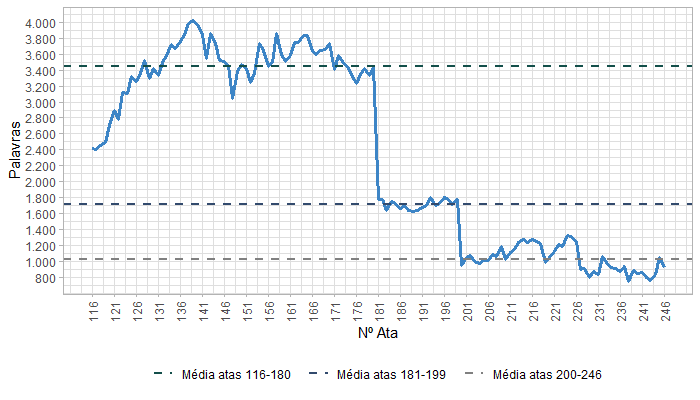
\includegraphics[scale = 0.75]{figuras/grafico_total_words.png}
	\fonte{Elaboração do autor.}
\end{figure}

A alteração do tamanho a partir da ata 181 veio por retirada relevante de seções nos comunicados, onde o cargo de presidência do BCB estava ocupado por Alexandre Tombini. Por fim, a última quebra é referente a ata de número 200 em diante, onde a presidência do BCB se encontrava sob o comando de Ilan Goldfajn, em que houveram mudanças significativas nas estruturas e seções dos comunicados. Vale ressaltar que a quantidade de palavras nas atas do Copom não necessariamente está relacionado a maior qualidade das informações. Neste caso, a redução dos comunicados temporalmente é, em definitivo, uma questão interessante de ser abordada, ainda mais quando o tocante é legibilidade, transparência e credibilidade (maiores detalhes abordados em \citeonline{Omotosho2019}).

Outra questão interessante que merece atenção é em relação as palavras mais frequentes (absolutamente falando) nas atas do Copom em todo o período analisado, conforme a Figura \ref{figure:wordcloud} apresenta, sendo que quanto maior a disposição da palavra, mais frequentemente ela é observada. 

De antemão, destaca-se termos como \textit{'inflation'}, \textit{'prices'}, \textit{'rate'}, \textit{'monetary + policy'}, \textit{'market + expectations'}, entre outras palavras relevantes. Vale notar-se também a alta correlação de $0,81$ entre os termos \textit{'inflation'} e \textit{'increased'}, denotando um alto aparecimento conjunto dessas palavras, isto é, aumento da inflação é um tópico muito recorrente nas atas do Copom, conforme o esperado.

Tais palavras estão em consonância com os objetivos tanto principais como secundários de um Banco Central, isto é, foco na estabilidade de preços, nível de atividade econômica e sinais acerca de políticas posteriores, fornecendo expectativas ao mercado \cite{blinder2000central, mishkin2000, bernanke2004monetary}.

\begin{figure}[hbtp]
	\centering
	\caption{Núvem de palavras mais frequentes nas atas} \label{figure:wordcloud}
	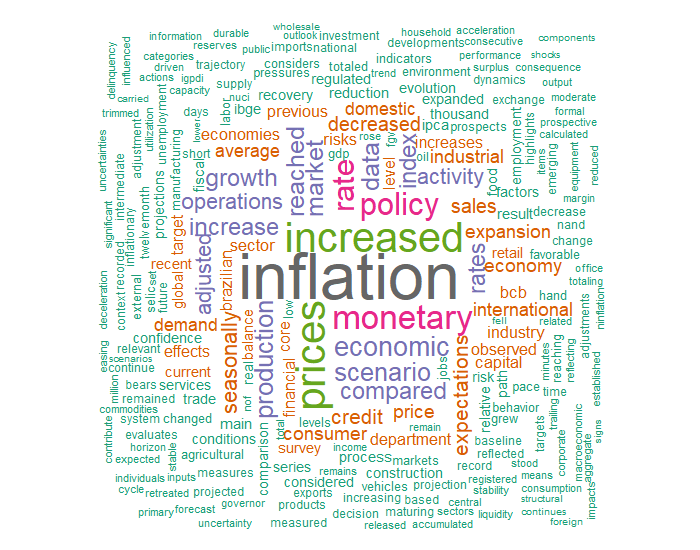
\includegraphics[scale = 0.75]{figuras/wordcloud_copom_words.png}
	\fonte{Elaboração do autor.}
\end{figure}

Após ter-se visualizado de forma ampla os termos mais recorrentes englobando todas as atas desde janeiro de 2006 até maio de 2022, separou-se as palavras que mais apareceram em cada ata. Como por exemplo, conforme observado na Figura \ref{figure:absolut_freq_words}, tem-se as oito palavras mais frequentes de uma sub-amostra, da ata 235 até a ata 246. Tal qual o esperado e apontado anteriormente pela Figura \ref{figure:wordcloud}, \textit{'inflation'} é o termo que aparece como mais corriqueiro para todas as atas, confirmado pelas atas da sub-amostra. Termos como \textit{'monetary'}, \textit{'scenario'}, \textit{'policy'}, \textit{'economic'} e \textit{'rate'} também são homogeneamente comuns. Detalhe para o surgimento no pódio entre as oito mais citadas da palavra \textit{'risks'} na ata 236 até a ata 242, saindo e reaparecendo na ata 246.

\begin{figure}
	\centering
	\caption{Palavras mais frequentes nas atas do Copom (atas nº 235 até nº 246)} \label{figure:absolut_freq_words}
	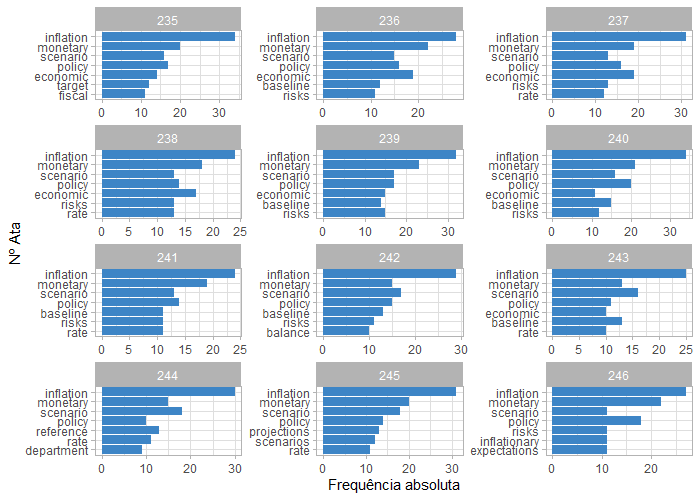
\includegraphics[scale = 0.75]{figuras/words_frequency_copom_text.png}
	\fonte{Elaboração do autor.}
\end{figure}

De qualquer maneira, apesar de ser interessante a reafirmação dos termos discutidos nas atas em relação aos objetivos de um comunicado de fonte oficial desta grandeza, pode-se constatar que em linhas gerais as palavras se repetem muito. Uma maneira de contornar essa questão e tentar extrair as palavras com maior importância de cada ata, é tornar a atenção para as frequências dos termos (\textit{tf}) em relação à frequência inversa do documento (\textit{idf}), denominada estatística tf-idf, abordada anteriormente na seção metodológica.

Como enunciado em \citeonline{silge2017text}, a parte \textit{idf} desta relação de frequências diminui o peso para palavras que aparecem muitas vezes nos documentos e aumenta o peso para palavras que não aparecem muitas vezes, sendo que uma vez multiplicado pela parte \textit{tf} nos resulta na frequência do termo ajustado por quão raramente ele aparece nos comunicados, isto é, extrai-se as palavras mais relevantes para cada ata dentro do período de análise proposto.

\begin{figure}
	\centering
	\caption{Frequências relativas, visualização das caudas longas (atas nº 238 até nº 246)} \label{figure:relative_freq_histograms}
	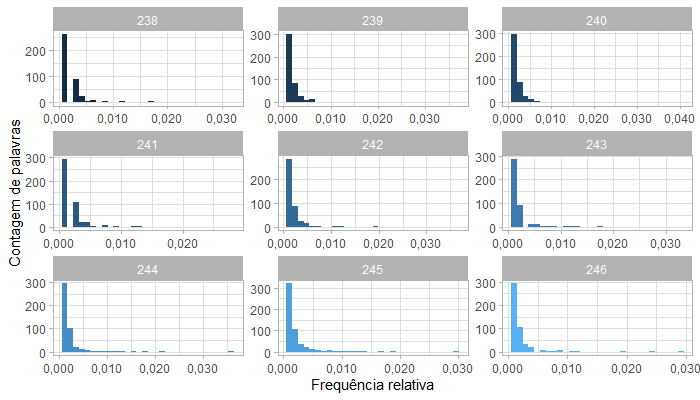
\includegraphics[scale = 0.75]{figuras/histogram_freq_words.png}
	\fonte{Elaboração do autor.}
\end{figure}

Mediante demonstrado pelos histogramas na Figura \ref{figure:relative_freq_histograms}, por meio da frequência relativa (número de vezes que determinada palavra aparece em determinada ata dividido pelo número de palavras naquela ata) pode-se perceber que existem muitos termos nas caudas da distribuição (que aparecem poucas vezes), sendo assim, poucas palavras que aparecem muitas vezes e muitas palavras que aparecem poucas vezes.

Salienta-se que distribuições de cauda longa como as representadas na Figura \ref{figure:relative_freq_histograms}, são comuns no estudo estatístico-linguístico dado um \textit{Corpus} (neste caso os documentos das atas do Copom), onde há uma relação inversamente proporcional entre a frequência em que determinada palavra aparece e o rank (ordenação da maior para menor frequência) dessa mesma palavra. A versão clássica dessa relação é chamada Lei de Zipf \cite{piantadosi2014zipf}.

\begin{table}[hbtp]
	\centering
	\caption{Estatísticas \textit{tf-idf} para palavras da ata nº 246} \label{table:tf_idf}
	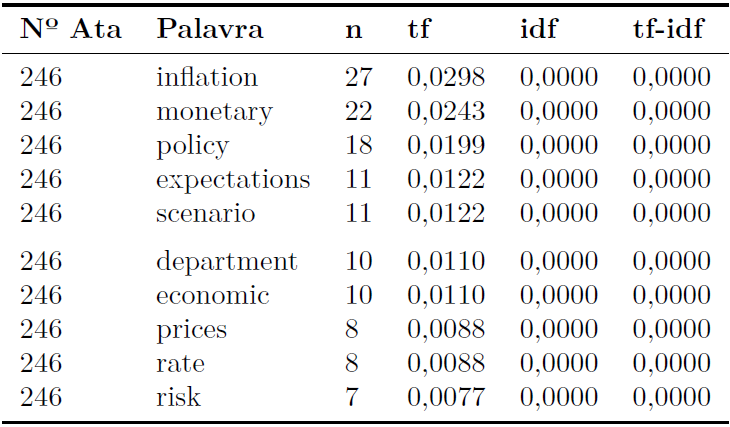
\includegraphics[scale = 0.50]{figuras/tabela_tf_idf.PNG}
	\fonte{Elaboração do autor.}
\end{table}

Tomando a ata nº 246 como exemplo, conforme apresentado na Tabela \ref{table:tf_idf}, tem-se a palavra, a quantidade de vezes que ela aparece na determinada ata, a frequência do termo (\textit{tf}), frequência inversa do documento (\textit{idf}) e a estatística \textit{tf-idf}. Como é possível contemplar, para palavras que são muito comuns entre todas as atas (\textit{'inflation'}, \textit{'expectations'}, \textit{'prices'} etc.), a \textit{idf} será zero (e por consequência a estatística \textit{tf-idf} também), uma vez que $\ln(1) = 0 $.

Já, quando olha-se para as maiores estatísticas \textit{tf-idf}, por exemplo, da ata nº 227 até a ata nº 246, consoante a Figura \ref{figure:tf_idf}, tem-se resultados muito promissores e interessantes. Primeiramente, percebe-se de forma notória que as palavras se diferem bastante entre si e em relação àquelas presentes na Figura \ref{figure:absolut_freq_words}. 

\begin{figure}[hbtp]
	\centering
	\caption{Estatísticas \textit{tf-idf} (atas nº 227 até nº 246)} \label{figure:tf_idf}
	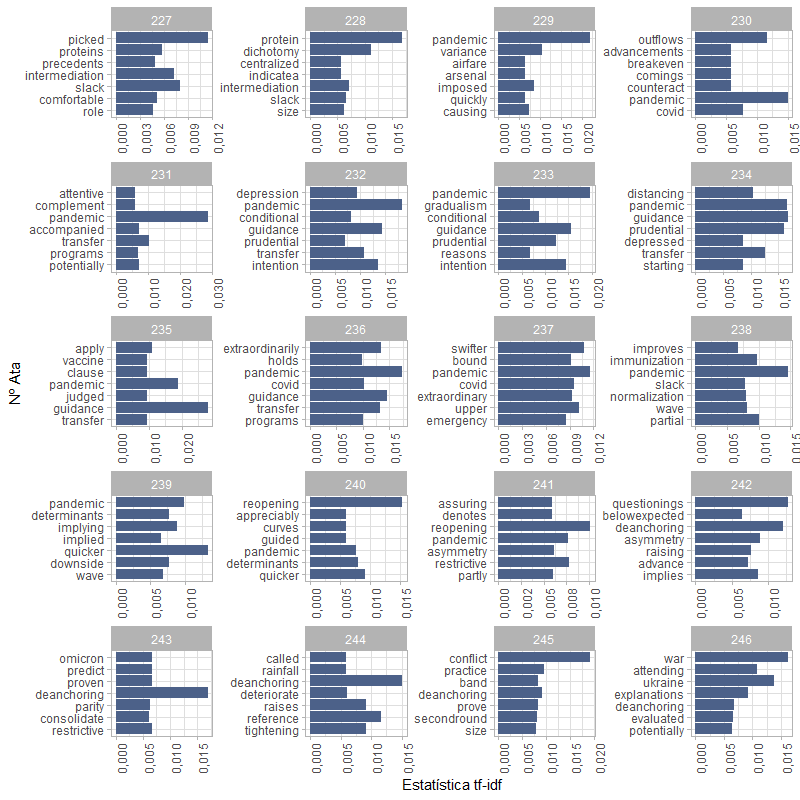
\includegraphics[scale = 0.75]{figuras/tf_idf_copom_text_refined.png}
	\fonte{Elaboração do autor.}
\end{figure}

Além disso, se nota não só o surgimento da palavra \textit{'pandemic'} a partir da ata nº 229, como sua persistência até a ata 240, com alta relevância. Na ata nº 229, pode-se perceber o aparecimento da palavra \textit{'airfare'} (referente à variação nos preços de passagens aéreas devido à retração do preço internacional do barril de petróleo), assim como a palavra \textit{'imposed'}, em relação às restrições impostas; ambas referências como consequência do estourar da pandemia do Coronavírus em 2020. 

Na ata nº 230, tem-se o surgimento da palavra \textit{'outflows'}, referente a fortes saídas de capital no Brasil (um país emergente) em momentos incertos e de alto risco financeiro. Também rassalta-se o surgimento de \textit{'transfer + programs'} na ata nº 231, acerca da implementação de programas de crédito e transferência de renda a famílias vulneráveis. No intermédio, destacam-se termos como \textit{'prudential'}, \textit{'gradualism'}, \textit{'distancing'}, \textit{'vaccine'}, \textit{'emergency'}, \textit{'immunization'}, \textit{'partial + normalization'}, \textit{'restrictive'}, \textit{'omicron'}, todos relacionados à crise sanitária. 

Outrossim, observa-se na ata 240, a inauguração do termo \textit{'reopening'} em alusão ao início da reabertura da economia como um todo. Atenta-se também para o surgimento de \textit{'deanchoring'} na ata nº 242 (perdurando até a 246), tratando-se da desancoragem das expectativas de inflação. Por fim, tem-se termos como \textit{'conflict'} e \textit{'ukraine'} devido à invasão da Ucrânia por parte da Rússia, iniciada em fevereiro de 2022.

Feitas análises de estatísticas descritivas referente ao período proposto, categorizou-se as palavras presentes nos documentos em positivas ou negativas e criou-se um índice de sentimentos das atas do Copom.

\section{Índice de sentimentos das Atas do Copom} \label{section:indice_sentimentos}

No presente trabalho, foi utilizado o dicionário léxico proposto por \citeonline{bing_liu_2004}, que conta com 6.786 palavras classificadas com teor positivo ou negativo, onde alguns desses termos podem ser observados na Tabela \ref{table:bing_liu}. É importante destacar que esse método desconsidera bigramas (\textit{'no good'}, \textit{'not true'}, \textit{'no risks'}, \textit{'no volatility'}), ou seja, ele é baseado somente em unigramas, que são palavras isoladas \cite{silge2017text}.

\begin{table}[hbtp]
	\centering
	\caption{Palavras presentes no dicionário de sentimentos proposto por \citeonline{bing_liu_2004}} \label{table:bing_liu}
	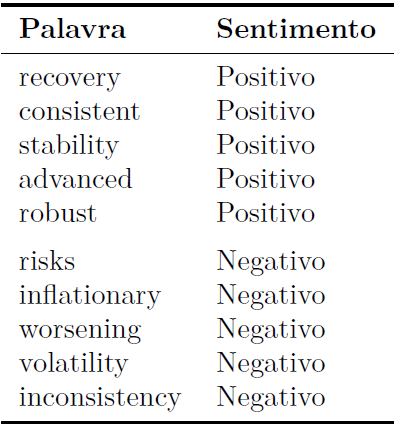
\includegraphics[scale = 0.50]{figuras/palavras_hu_liu2004.PNG}
	\fonte{Elaboração do autor.}
\end{table}

Cruzando as informações das atas do Copom que foram adquiridas por meio da raspagem de dados \textit{web} e posteriormente tratadas, com as informações presentes no dicionário léxico, encontrou-se o número de palavras categorizadas como positivas e negativas para cada documento de texto. 

\begin{table}[hbtp]
	\centering
	\caption{Sentimentos encontrados nas atas do Copom} \label{table:sentiment_index}
	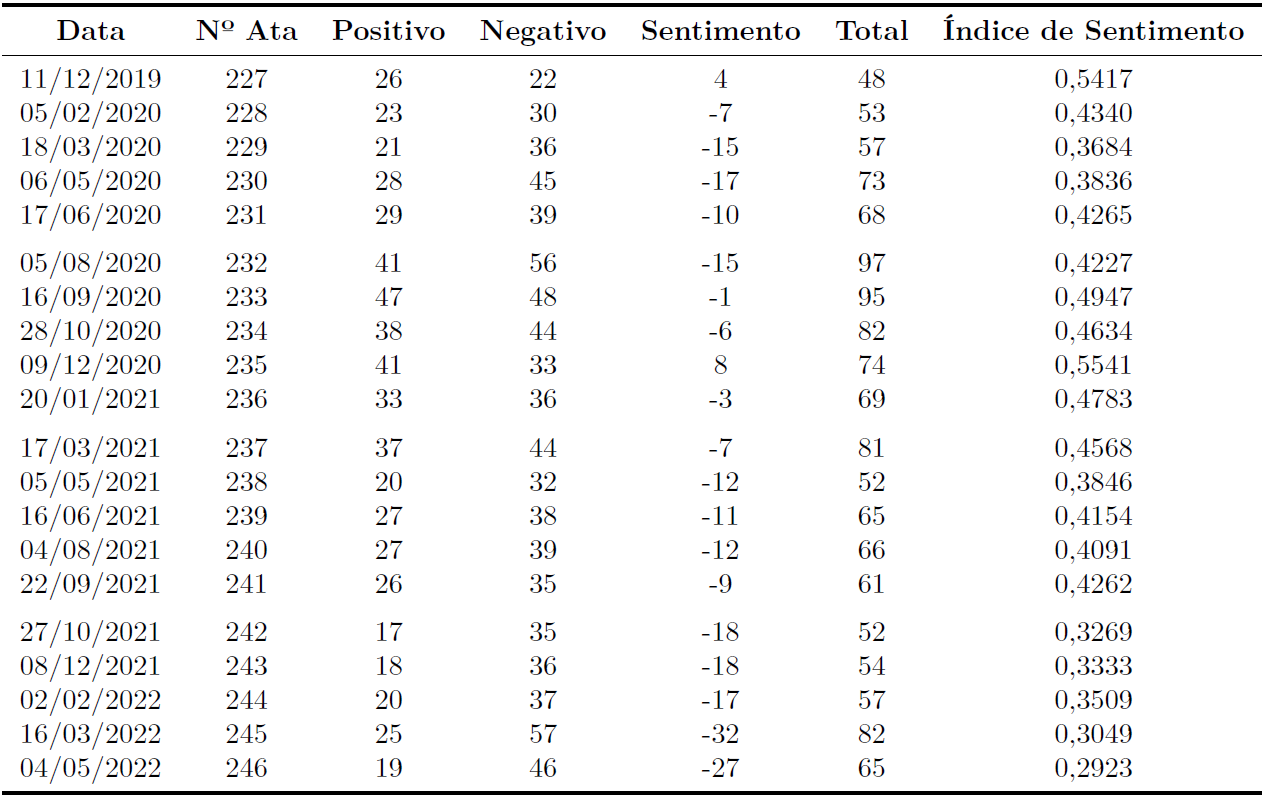
\includegraphics[scale = 0.45]{figuras/tabela_sentimento.PNG}
	\fonte{Elaboração do autor.}
\end{table}

Pós cruzamento dos dados e categorização das palavras, se baseando em \citeonline{bholat_etal2015}, criou-se o índice de sentimentos a seguir:

\begin{ceqn}
\begin{align} \label{eq:eq_sentiment_index}
 IS_{t} = \frac{NP_{t}}{NP_{t} - NN_{t}} 
\end{align}
\end{ceqn} onde, na equação \eqref{eq:eq_sentiment_index}, tem-se que $IS_{t}$ é o índice de sentimento para a ata no tempo $t$; $NP_{t}$ é a quantidade de palavras categorizadas como positivas para a ata no tempo $t$; e $NN_{t}$ é a quantidade de palavras categorizadas como negativas para a ata no tempo $t$.

Sendo assim, como $0 \leq IS_{t} \leq 1$, quando o valor for acima de $0,5$ tem-se uma perspectiva otimista para a economia, caso contrário, temos a definição do sentimento de pessimismo. Destaca-se também que quanto mais próximo de $1$ o valor, mais otimista a ata, assim como quanto mais próximo de $0$, mais pessimista.

Para exemplificar, na Tabela \ref{table:sentiment_index}, estão dispostas informações do índice de sentimentos criado, da ata nº 227 até a de nº 246. A coluna \textit{Positivo} é o $NP_{t}$, a coluna \textit{Negativo} o $NN_{t}$, a coluna \textit{Sentimento} é o saldo (positivas subtraídas das negativas), a coluna \textit{Total} é a soma das palavras categorizadas e a última coluna é referente ao índice. Como é possível observar, das atas presentes na tabela, somente a 227 e 235 tiveram um saldo tido como otimista (e com baixo grau, de $0,5417$ e $0,5541$ respectivamente), o restante teve um teor negativo, com destaque para a ata nº 246 com um $IS_{246} = 0,2923$. 

\begin{figure}[hbtp]
	\centering
	\caption{Índice de sentimento das atas do Copom} \label{figure:sentiment_index}
	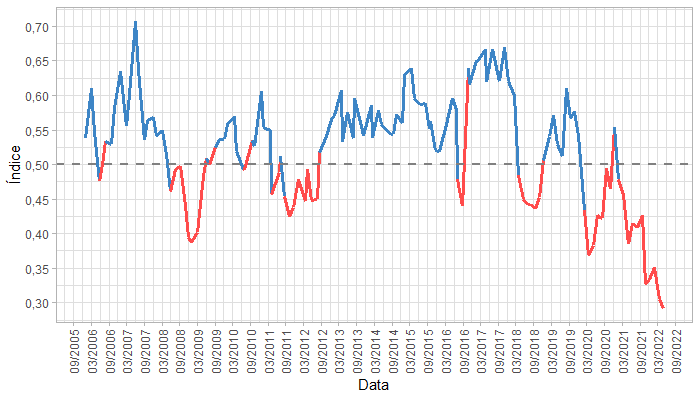
\includegraphics[scale = 0.75]{figuras/indice_de_sentimentos.png}
	\fonte{Elaboração do autor.}
\end{figure}

Por fim, foi elaborado um gráfico, conforme a Figura \ref{figure:sentiment_index}, com a série temporal do $IS_{t}$ criado, em que $t = 116,...,246$. A coloração da linha em azul representa períodos com um $IS_{t} > 0,5$ e a coloração em vermelho, um $IS_{t} \leq 0,5$. Na maior parte do tempo (82 das atas), observa-se o índice indicando teor positivo, enquanto no restante, inclusive para o período mais recente, nota-se o teor negativo (49 das atas).

Chega-se na conclusão de que, de forma geral, o Copom aborda seus comunicados acerca da condução de política monetária e assuntos relacionados à atividade e conjuntura econômica no Brasil de maneira otimista. Com o índice elaborado, comparou-se ele com variáveis macroeconômicas de interesse.

\subsection{Comparando o índice com variáveis macroeconômicas}

Assim como nos exercícios realizados por \citeonline{bloom2009uncertainty} e \citeonline{ferreira2017incerteza}, para as séries do Índice de Sentimentos, IBC-Br e PIM-PF foram extraídos os componentes cícliclos por meio do filtro de \citeonline{hp_filter1997}.

\begin{figure}[hbtp]
	\centering
	\caption{Séries macroecônomicas pós-tratamento} \label{figure:series_macro}
	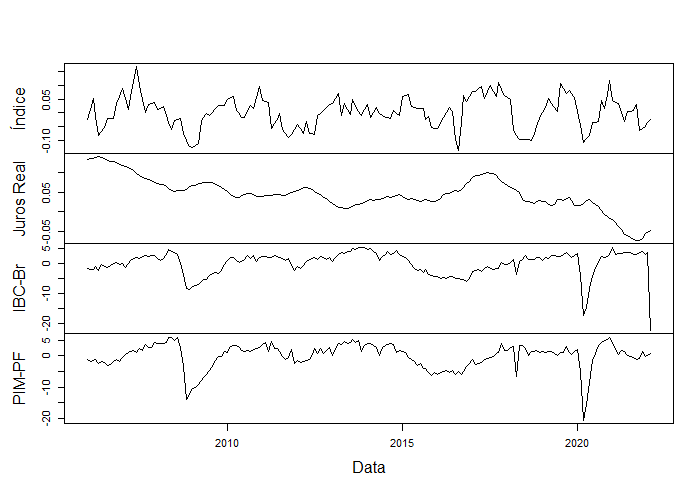
\includegraphics[scale = 0.75]{figuras/graf_series_macro.png}
	\fonte{Elaboração do autor.}
\end{figure}

A Figura \ref{figure:series_macro} demonstra as séries temporais das quatro variáveis que posteriormente serão inclusas no modelo VAR. Atenta-se para o fato de que o índice de sentimentos criado aparenta acompanhar as demais variáveis selecionadas em momentos críticos na economia, como, por exemplo, em 2008 com a Crise Financeira do Subprime e em 2020 com a Crise Sanitária do Covid-19. Além disso, é possível observar uma tendência de queda da taxa de juros real em nível, enquanto as demais séries aparentam ser estáveis.

\section{Resultados dos testes de estacionariedade} \label{section:testes_estac}

Conforme mencionado anteriormente, as variáveis inclusas em modelos VAR($p$) precisam possuir a característica de estacionariedade. Dessa maneira, foram realizados testes de raiz unitária de Dickey-Fuller (DF) e Dickey-Fuller Aumentado (ADF) - com uma defasagem - e de Kwiatkowski–Phillips–Schmidt–Shin (KPSS). 

\begin{table}[hbtp]
	\centering
	\caption{Resultados dos testes ADF sem constante e sem tendência} \label{table:adf_none}
	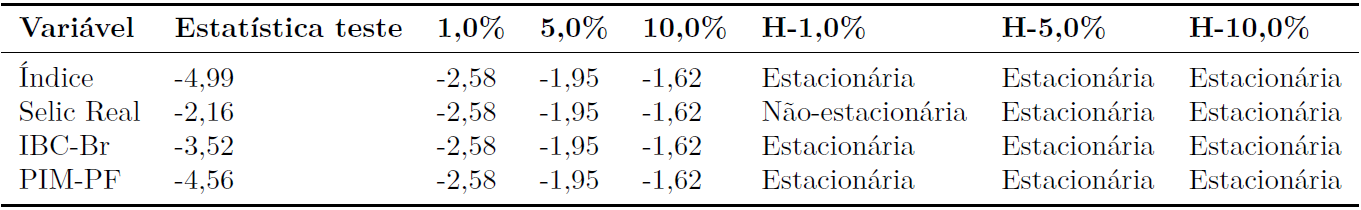
\includegraphics[scale = 0.40]{figuras/teste_adf_none.PNG}
	\fonte{Elaboração do autor.}
\end{table}

Primeiramente, conforme observa-se na Tabela \ref{table:adf_none}, elaborou-se o teste de ADF sem constante e sem tendência. A primeira e segunda coluna representam a variável e sua respectiva estatística do teste; já as colunas "$1,0\%$", "$5,0\%$" e "$10,0\%$" representam os níveis de significância ($\alpha$); e por fim as colunas "H-$1,0\%$", "H-$5,0\%$" e "H-$10,0\%$" indicam se a série é estacionária ou não através da aceitação ou não da hipótese nula. 

Por meio deste teste constata-se que praticamente todas as séries rejeitam a hipótese nula ($H_{0}$) de não-estacionariedade, portanto são estacionárias para todos os níveis de significância propostos, exceto para a série dos juros reais a um $\alpha = 1,0\%$.

\begin{table}[hbtp]
	\centering
	\caption{Resultados dos testes ADF com constante} \label{table:adf_drift}
	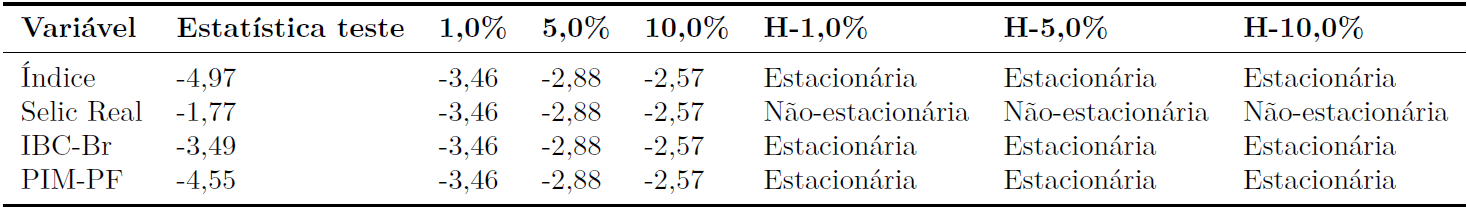
\includegraphics[scale = 0.40]{figuras/teste_adf_drift.PNG}
	\fonte{Elaboração do autor.}
\end{table}

Quando feito o teste de ADF com constante, conforme a Tabela \ref{table:adf_drift} demonstra, a série dos juros reais não só é tida como não-estacionária a um $\alpha = 10,0\%$, mas como para $\alpha = 5,0\%$ e $\alpha = 1,0\%$ também.

Elaborando o teste de ADF com constante e tendência, como contempla-se na Tabela \ref{table:adf_trend}, além das taxas de juros reais não serem estacionárias, tem-se que para níveis de significância de $5,0\%$ e $1,0\%$, o IBC-Br também apresenta não-estacionariedade.

\begin{table}[hbtp]
	\centering
	\caption{Resultados dos testes ADF com constante e com tendência} \label{table:adf_trend}
	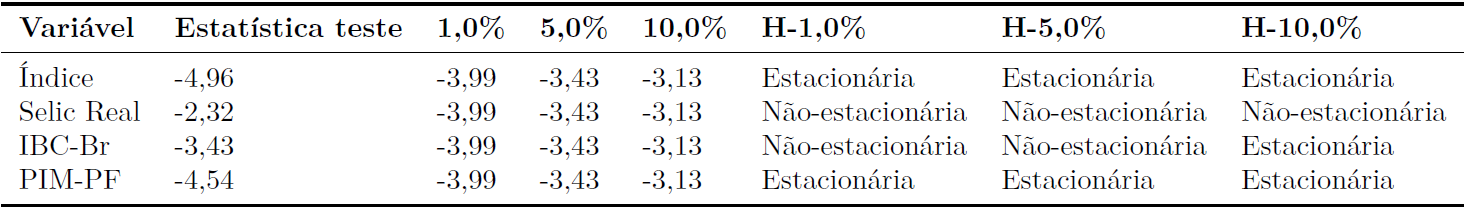
\includegraphics[scale = 0.40]{figuras/teste_adf_trend.PNG}
	\fonte{Elaboração do autor.}
\end{table}

Por fim, por meio do teste de KPSS, em que a hipótese nula ($H_{0}$) é a de estacionariedade, tem-se que somente a série das taxas de juros reais rejeita $H_{0}$, conforme está disposto na Tabela \ref{table:kpss}.

\begin{table}[hbtp]
	\centering
	\caption{Resultados dos testes KPSS} \label{table:kpss}
	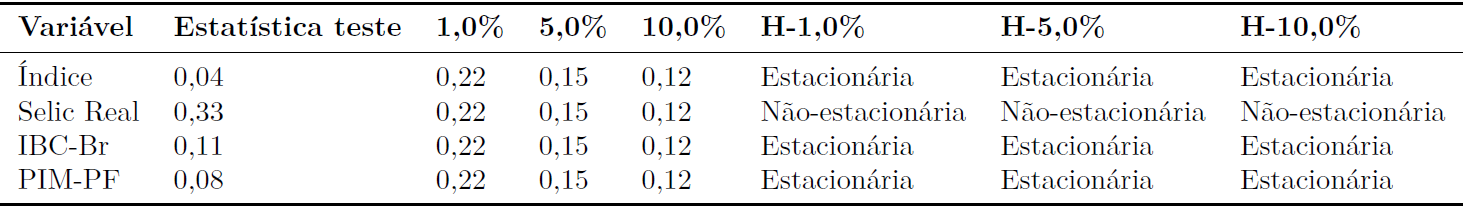
\includegraphics[scale = 0.40]{figuras/teste_kpss.PNG}
	\fonte{Elaboração do autor.}
\end{table}

\pagebreak{}

Desta maneira, optou-se por manter todas as séries em seus níveis, exceto para a série dos juros reais, em que foi feita uma diferenciação, como pode ser observado na Figura \ref{figure:series_macro_2}.

\begin{figure}[hbtp]
	\centering
	\caption{Séries macroeconômicas pós-tratamento, com juros real diferenciado} \label{figure:series_macro_2}
	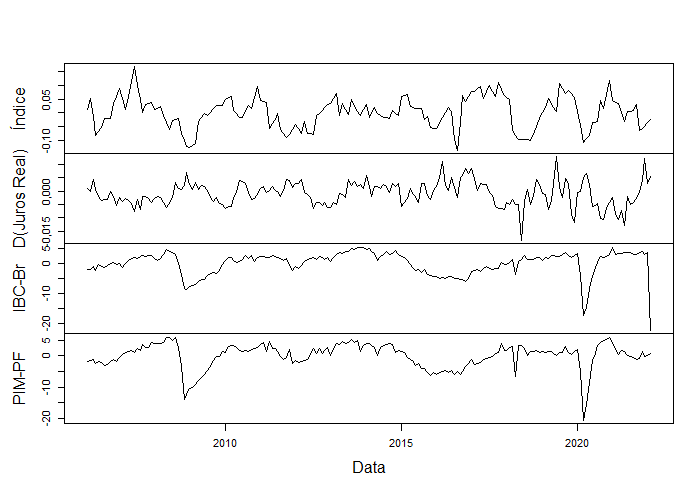
\includegraphics[scale = 0.75]{figuras/graf_series_macro_2.png}
	\fonte{Elaboração do autor.}
\end{figure}

Após isso, todos os testes foram refeitos e para um $\alpha = 5,0\%$, que é o nível de significância desejado, constatou-se que todas as séries são estacionárias, prontas para serem inclusas no modelo VAR.

%\subsection{Dickey-Fuller Aumentado (ADF)}

%\subsection{Phillips-Perron (PP)}

%\subsection{Kwiatkowski–Phillips–Schmidt–Shin (KPSS)}

%\section{Resultados dos testes de cointegração}

%\section{Resultados do mecanismo de correção de erros (MCE)}

\section{Resultados do modelo de vetores autorregressivos (VAR)} \label{section:VAR}

Detendo o conjunto de variáveis estacionárias, a estimação do modelo VAR($p$) pode ser efetuada, onde os critérios de decisão abordados nas Equações \eqref{eq:BIC}, \eqref{eq:AIC} e \eqref{eq:HQ} são utilizados para se definir as ordens ótimas de defasagens. Após isso, visto que a estabilidade do modelo e de seus parâmetros foram garantidas, foi selecionada a ordem que apresentou os melhores testes de diagnóstico.

A partir dos critérios $BIC(p,q)$ e $HQ(p,q)$ o número de defasagens ótimo apontado foi de 1, enquanto para o critério $AIC(p,q)$ o número aumenta para 2. Dessa forma, foram estimados dois modelos, contemplando as duas possibilidades de defasagens propostas pelos critérios de informação. Tanto para uma quanto para duas defasagens, as raízes do polinômio característico ficaram abaixo de um, ou seja, fora do círculo unitário, além dos testes de flutuação empírica, abordado em \citeonline{ploberger1992cusum}, evidenciarem parâmetros estáveis, isto é, sem quebras estruturais (os resultados podem ser constatados no Apêndice A).

%No modelo de VAR($1$), para a equação do índice de sentimentos o coeficiente de determinação ajustado foi de $R_{adj}^2 = 0,659$; enquanto que para a equação da taxa de juros real diferenciada, o $R_{adj}^2 = 0,416$. Para a equação da atividade econômica, obteve-se um $R_{adj}^2 = 0,623$; ao passo que a equação da produção industrial resultou num $R_{adj}^2 = 0,697$, sendo o maior entre todos. 

Para o modelo VAR($1$), o teste conjunto de autocorrelação serial de Breusch-Godfrey falhou, dado que o p-valor = $0,007$, abaixo de p-valor = $0,05$. Considerando os testes individuais, somente a série do D(Juros Real) e a série do IBC-Br entregaram um p-valor > $0,05$. Enquanto, para o teste conjunto ARCH de heterocedasticidade, o modelo apresentou estar estável, já que retornou um p-valor = $0,10$.

Dessa maneira, optou-se trabalhar com o VAR($2$), onde o teste conjunto de autocorrelação serial de Breusch-Godfrey apresentou como p-valor = $0,10$, acima de p-valor = $0,05$, denotando assim que não há autocorrelação nos resíduos das séries do modelo estimado. Considerando os testes individuais, todas as séries apresentaram um p-valor > $0,05$, isto é, individualmente também não apresentam correlação serial. Enquanto que, para o teste conjunto ARCH de heterocedasticidade, o modelo apresentou estar estável, retornando um p-valor = $0,10$.

No VAR($2$), considerando todas as variáveis como endógenas, obteve-se então o seguinte sistema de equações:

\begin{ceqn}
\begin{align} \label{eq:sist_equacoes_var_2}
&IS_{t} = IS_{t-1} + \Delta JR_{t-1} + AE_{t-1} + PI_{t-1} + IS_{t-2} + \Delta JR_{t-2} + AE_{t-2} + PI_{t-2} + \epsilon_{IS_{t}} \\
&\Delta JR_{t} = IS_{t-1} + \Delta JR_{t-1} + AE_{t-1} + PI_{t-1} + IS_{t-2} + \Delta JR_{t-2} + AE_{t-2} + PI_{t-2} + \epsilon_{\Delta JR_{t}} \\
&AE_{t} = IS_{t-1} + \Delta JR_{t-1} + AE_{t-1} + PI_{t-1} + IS_{t-2} + \Delta JR_{t-2} + AE_{t-2} + PI_{t-2} + \epsilon_{AE_{t}} \\
&PI_{t} = IS_{t-1} + \Delta JR_{t-1} + AE_{t-1} + PI_{t-1} + IS_{t-2} + \Delta JR_{t-2} + AE_{t-2} + PI_{t-2} + \epsilon_{PI_{t}}
\end{align}
\end{ceqn} onde a equação do índice de sentimentos ($IS$) chegou a um coeficiente de determinação ajustado no valor de $R_{adj}^2 = 0,667$; ao passo que para a equação da taxa de juros real diferenciada ($\Delta JR$), o $R_{adj}^2 = 0,429$. Para a equação da atividade econômica ($AE$), resultou-se num $R_{adj}^2 = 0,626$; enquanto a equação da produção industrial ($PI$) decorreu em um $R_{adj}^2 = 0,722$, sendo o maior entre todos. Os coeficientes das equações podem ser vistos no Apêndice A.

\subsection{Causalidade de Granger}

%Para o modelo de VAR($1$), nos testes individuais de causalidade de Granger, nenhuma variável apresentou Granger-causar o índice de sentimentos criado para um nível de $\alpha = 5,0\%$. No sentido do índice Granger-causar as variáveis, apenas a atividade econômica e a produção industrial apresentaram rejeição à $H_{0}$ de não-causalidade, porém apenas para um $\alpha = 10,0\%$. Entretanto, para o teste conjunto de causalidade tem-se para todas as variáveis um p-valor > $0,05$, dessa forma rejeitando a hipótese nula de não-causalidade, ou seja, todas as variáveis Granger-causam o índice de sentimentos.

No modelo VAR($2$), para os testes individuais de causalidade de Granger, nenhuma variável apresentou Granger-causar o índice de sentimentos criado para um nível de $\alpha = 5,0\%$. Considerando o índice Granger-causar as variáveis, conforme observa-se na Tabela \ref{table:granger_individual_model2}, tem-se que apenas a PIM-PF é afetada, para um $\alpha = 5,0\%$, sendo seu p-valor = $0,02$.

\begin{table}[hbtp]
	\centering
	\caption{Testes individuais de causalidade de Engle-Granger para o VAR($2$)} \label{table:granger_individual_model2}
	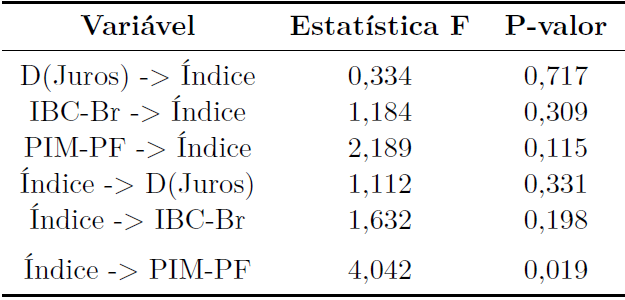
\includegraphics[scale = 0.45]{figuras/granger_individual_model2.PNG}
	\fonte{Elaboração do autor.}
\end{table}

Para o teste em conjunto de causalidade de Granger, como apresentado na Tabela \ref{table:granger_conjunto_model2}, tem-se um p-valor > $0,05$ para as variáveis da diferença da taxa de juros real e produção industrial, assim essas variáveis não Granger-causam o índice e as outras variáveis, apesar de que para a atividade econômica o p-valor = $0,04$, fazendo com que o IBC-Br possa Granger-causar o índice criado, tanto quanto as outras variáveis, ou todas, entretanto como visto no teste individual, o IBC-Br não Granger-causa o índice.

\begin{table}[hbtp]
	\centering
	\caption{Teste conjunto de causalidade de Engle-Granger para o VAR($2$)} \label{table:granger_conjunto_model2}
	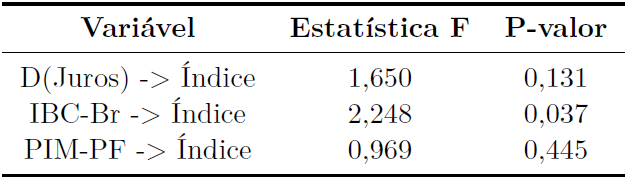
\includegraphics[scale = 0.50]{figuras/granger_conjunto_model2.PNG}
	\fonte{Elaboração do autor.}
\end{table}

\subsection{Funções impulso-resposta (IRF)}

A análise das Funções de Impulso-Resposta demonstrou, conforme a Figura \ref{figure:irf_indice_indice_model_2} aponta que, dado um choque positivo no índice, a resposta do próprio índice sofre positivamente com impacto decrescente, segundo o tamanho do choque dado, de forma significativa. Salienta-se que para o VAR($2$), a partir do 6º período, o choque deixa-se de ser significante para um intervalo de confiança de $95,0\%$.

\begin{figure}[hbtp]
	\centering
	\caption{IRF do VAR($2$): Índice $\rightarrow$ Índice} \label{figure:irf_indice_indice_model_2}
	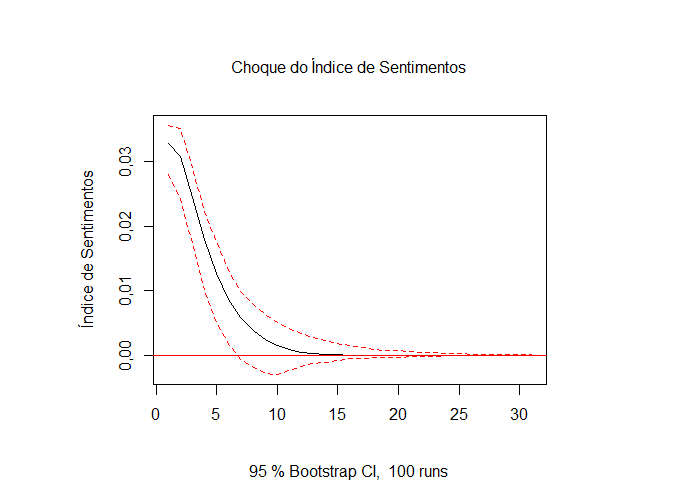
\includegraphics[scale = 0.60]{figuras/irf_indice_indice_model_2.PNG}
	\fonte{Elaboração do autor.}
\end{figure}


Já, a partir de um choque efetuado no índice em relação à diferença dos juros reais, como observa-se na Figura \ref{figure:irf_indice_selic_model_2}, tem-se uma resposta negativa até o 4º período (sendo este um ponto de inflexão), aumentado com o passar dos períodos. Entretanto, para o VAR($2$), o choque é somente significativo entre o 4º e 5º período, para $95,0\%$ de confiança.

\begin{figure}[hbtp]
	\centering
	\caption{IRF do VAR($2$): Índice $\rightarrow$ D(Juros)} \label{figure:irf_indice_selic_model_2}
	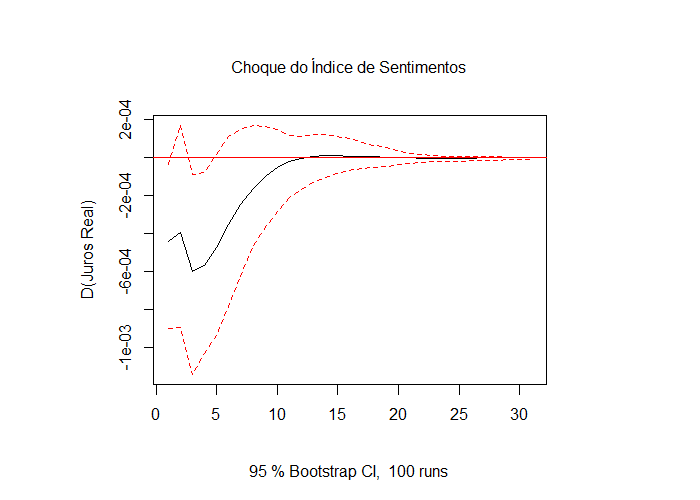
\includegraphics[scale = 0.60]{figuras/irf_indice_selic_model_2.PNG}
	\fonte{Elaboração do autor.}
\end{figure}

Outrossim, quando se atenta à resposta da atividade econômica dado um choque no índice de sentimentos, percebe-se conforme a Figura  \ref{figure:irf_indice_ibcbr_model_2} aponta, que os impactos são sentidos a partir do 2º mês, perdurando significativamente (intervalo de confiança de $95,0\%$) até o 5º período para o VAR($2$). Do choque até o quinto período, tem-se uma reação positiva, sendo que a partir do 5º, ela decai.

\begin{figure}[hbtp]
	\centering
	\caption{IRF do VAR($2$): Índice $\rightarrow$ IBC-Br} \label{figure:irf_indice_ibcbr_model_2}
	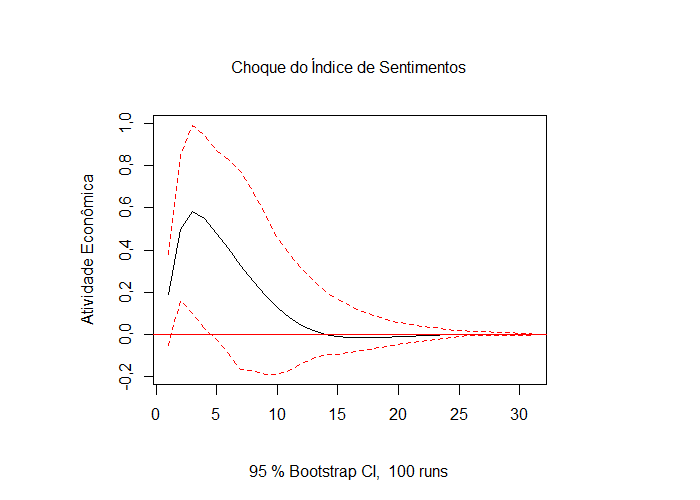
\includegraphics[scale = 0.60]{figuras/irf_indice_ibcbr_model_2.PNG}
	\fonte{Elaboração do autor.}
\end{figure}

Por fim, dado um impulso no índice, a resposta da produção industrial se assemelha com a da atividade econômica, onde como se observa na Figura \ref{figure:irf_indice_pimpf_model_2}, há um pico no 5º período, onde a partir dele, os choques deixam de ser significativos.

\begin{figure}[hbtp]
	\centering
	\caption{IRF do VAR($2$): Índice $\rightarrow$ PIM-PF} \label{figure:irf_indice_pimpf_model_2}
	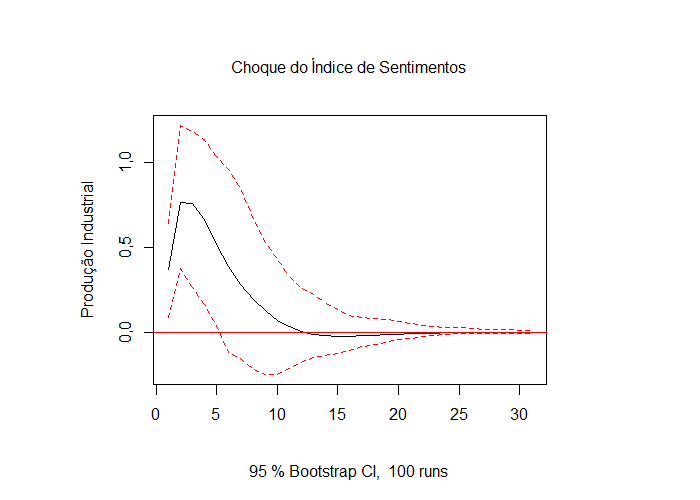
\includegraphics[scale = 0.60]{figuras/irf_indice_pimpf_model_2.PNG}
	\fonte{Elaboração do autor.}
\end{figure}

Em \citeonline{ferreira2017incerteza}, são disponibilizados apenas os resultados das IRF de atividade econômica e produção industrial, dado um choque no IIE-Br, onde ambas respondem negativamente, com pequenos intervalos significantes, semelhantes aos resultados do trabalho de \citeonline{bloom2009uncertainty}. As possíveis divergências com os resultados obtidos neste trabalho, provavelmente se dão, pois, os autores criaram índices de incerteza da economia e não um índice de sentimentos das atas do Copom. Não só isso, os autores contemplaram um número maior de variáveis, como câmbio, desemprego e preços de commodities, além de impor uma restrição de ordenamento das variáveis, o que ia além da proposta deste trabalho. Interessante apontar que, por ainda serem incipientes os estudos que relacionam mineração textual, análise de sentimentos e economia, os resultados podem servir como norteadores de alguma forma.

Dessa maneira, conclui-se que por meio de choques aos sentimentos dos comunicados das atas do Copom, a diferença da taxa de juros básica acumulada em doze meses, descontada da taxa de inflação (também acumulada em doze meses), sofre negativamente, ao qual se estabiliza conforme se avança nos períodos. Entretanto, quando se olha para a atividade econômica e para a produção industrial, percebe-se que a resposta é positiva com impactos decrescentes, também se estabilizando em torno de zero conforme o avanço do tempo, visto que os choques não possuem efeitos permanentes em séries temporais que possuem a característica de estacionariedade. 